\documentclass[tikz, border=50pt]{standalone}

\usepackage{tikz}
\usepackage{geometry}
\usepackage{medl_colors}
\usepackage{pgfplots}

\usetikzlibrary{shapes.multipart, shapes.geometric, arrows.meta}
\usetikzlibrary{matrix,decorations.pathreplacing, calc, positioning,fit}
\usetikzlibrary{positioning}

\pgfplotsset{compat=1.18}

\begin{document}
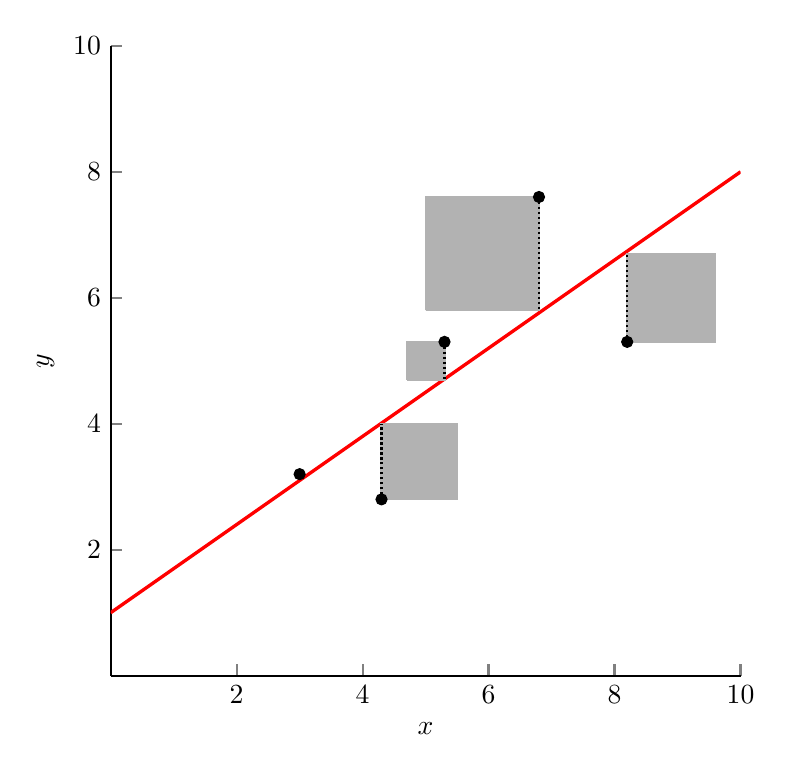
\begin{tikzpicture}

\newcommand\medlsquare[6]
{
    \coordinate (#4A) at (#1, #2);
    \coordinate (#4B) at (#1+#3, #2);
    \coordinate (#4C) at (#1+#3, #2+#3);
    \coordinate (#4D) at (#1, #2+#3);
    \filldraw[thick, draw=black!30,fill=black!30] plot coordinates {(#4A) (#4B) (#4C) (#4D) (#4A)};
    \filldraw [black] (#4#5) circle (2pt);
    \draw[thick, densely dotted] (#4#5) -- (#4#6);
}

\begin{axis}[
axis line style = thick,
xmin = 0, xmax = 10,
ymin = 0, ymax = 10,
xlabel={$x$}, 
ylabel={$y$},
xtick={2,4,6,8,10},
ytick={2,4,6,8,10},
tick style={thick},
xtick pos=bottom,
ytick pos=left,
x=.8cm,
y=.8cm,
axis lines* = left
]

\addplot[color = red, very thick] coordinates {(0, 1) (10, 8)};
\filldraw [black] (3,3.2) circle (2pt);
\medlsquare{4.3}{2.8}{1.2}{square}{A}{D}
\medlsquare{4.7}{4.7}{.6}{square}{C}{B}
\medlsquare{5}{5.8}{1.8}{square}{C}{B}
\medlsquare{8.2}{5.3}{1.4}{square}{A}{D}

\end{axis}
\end{tikzpicture}
\end{document}